	% Multiple Item Proof
	\subsection{Integrity Check}
	\label{sec:mip}
	\subsectionnames{Simon Fallnich}

		To verify the integrity of the data, which is sent from the client-side application to the smart contract, we utilize Merkle trees (see \autoref{subsec:merkle-tree}), where each data block of a Merkle tree corresponds to a state variable of the smart contract.
		Although the computations for constructing a Merkle tree are straightforward, the order, in which the given data blocks and hashes are concatenated, is crucial.
		Therefore, information about the position of the given data blocks and hashes in the resulting Merkle tree needs to be sent to the smart contract as well.
		In the following, we will summarize all data other than the root hash, which is required to verify the integrity of one or more given data blocks, under the term \emph{proof}.
		
		For the case of verifying one data block, a simple proof could consist of the data block, an array which contains the required hashes in the same order in which they are used in the computations, and an array of booleans of the same length, in which each boolean defines whether to concatenate a specific hash from the left or from the right side.
		Such a proof can be generated and verified without great effort and implementations are available.
		Nevertheless, this principle cannot be extended to support multiple data blocks in a single proof --- with this approach, each data block requires its own proof, which dramatically increases the overhead added by the integrity check mechanism.
		To minimize the overhead, we implemented an integrity check which enables the verification of multiple data blocks within a single proof, referred to as \emph{multiple item proof}.

		% Proof Generation
		\subsubsection*{Proof Generation}
		\label{subsec:mip-generation}

			To generate a multiple item proof, the client-side application first constructs a Merkle tree of \emph{all} existing data blocks.
			For this, an array is created, which represents the nodes of a full binary tree whose number of leaf nodes equal the number of all data blocks, stored in level order.\footnote{This data structure is sufficient to represent a binary tree as the parent's index of a node with index $i$ can be computed as $\lfloor\frac{(i - 1)}2\rfloor$ and the indices of the left and right childs can be computed with $2i + 1$ and $2i + 2$, respectively.} The hashes of the data blocks are inserted into the array and the remaining hashes are computed recursively to construct a Merkle tree.
			\autoref{fig:mip-1} visualizes the relation between the resulting array and the respresented Merkle tree for an exemplary proof with a total of four data blocks, $D_0$, $D_1$, $D_2$ and $D_3$.

			In the next step, a new array of booleans with the same length is created, in which each boolean represents whether the hash of the corresponding node has to be computed during the proof verification or not.
			The hashes which need to be computed are, on the one hand, the hashes of the data blocks (leaf nodes) which should be verified.
			On the other hand, the hashes of all (direct and indirect) parent nodes of these nodes need to be computed as well, as they depend on the previously unknown hashes of the respective data blocks.
			\autoref{fig:mip-2} shows the resulting array and the correlation to the represented Merkle tree for the exemplary proof with four data blocks, in which $D_1$ and $D_2$ should be verified.

			Subsequently, the hashes which are required for the proof are determined.
			For this, another array with the same structure is created an initialized with null values.
			The hashes are inserted for every node in the array of booleans which has a "false" value and a parent with a "true" value --- to compute the hash of the parent node, the hash of such a node has to be concatenated with the hash of its sibling and therefore is required, but does not need to be computed itself.
			\autoref{fig:mip-3} shows the resulting array of hashes for the previously mentioned example proof.

			Finally, to complete a multiple item proof, the actual data blocks which should be verified and the index of the first leaf node are included, which is used to determine whether an index refers to a leaf node in the proof verification process.
			The complete example proof with four data blocks, in which $D_1$ and $D_2$ should be verified, consist of the following:
			\begin{itemize}
				\item{\makebox[3.5cm]{Array of booleans:\hfill}} $[\textrm{true}, \textrm{true}, \textrm{true}, \textrm{false}, \textrm{true}, \textrm{true}, \textrm{false}]$
				\item{\makebox[3.5cm]{Array of hashes:\hfill}} $[\textrm{null}, \textrm{null}, \textrm{null}, H_3, \textrm{null}, \textrm{null}, H_6]$
				\item{\makebox[3.5cm]{Data blocks:\hfill}} $\{D_1, D_2\}$
				\item{\makebox[3.5cm]{Index of first leaf:\hfill}} $3$.
			\end{itemize}

			\begin{figure}
				\centering
				\begin{subfigure}[b]{0.4\linewidth}
					\centering
					$$
						[H_0, H_1, H_2, H_3, H_4, H_5, H_6]
					$$
					\vspace*{3em}
					\caption{Data structure.}
					\label{}
				\end{subfigure}%
				\begin{subfigure}[b]{0.6\linewidth}
					\centering
					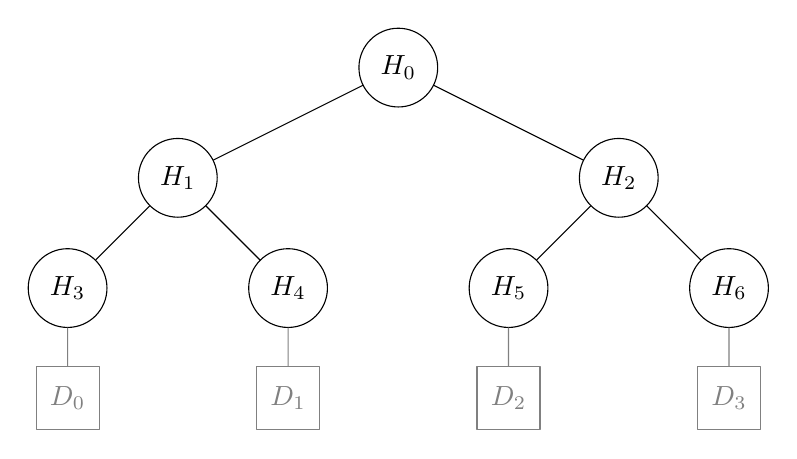
\begin{tikzpicture}[line cap=round, line join=round, scale=0.7]
						% First layer
						\node [circle, draw=black, fill=white, minimum size = 1cm] (node-1-1) at (0, 0) {$H_0$};
						% Second layer
						\foreach \a [count=\x] in {1, 2}
							\node [circle, draw=black, fill=white, minimum size=1cm] (node-2-\x) at (-12 + 8 * \x, -2) {$H_\a$};
						% Third layer
						\foreach \a [count=\x] in {3, ..., 6}
							\node [circle, draw=black, fill=white, minimum size=1cm] (node-3-\x) at (-10 + 4 * \x, -4) {$H_\a$};
						% First data layer
						\foreach \a [count=\x] in {0, ..., 3}
							\node [draw=gray, text=gray, fill=white, minimum size=0.8cm] (data-1-\x) at (-10 + 4 * \x, -6) {$D_\a$};
						% First layer arrows
						\foreach \a in {1, 2}
							\draw (node-1-1) -- (node-2-\a);
						% Second layer arrows
						\foreach \a in {1, 2}
							\draw (node-2-1) -- (node-3-\a);
						\foreach \a in {3, 4}
							\draw (node-2-2) -- (node-3-\a);
						\draw [draw=gray] (node-3-1) -- (data-1-1);
						\draw [draw=gray] (node-3-2) -- (data-1-2);
						\draw [draw=gray] (node-3-3) -- (data-1-3);
						\draw [draw=gray] (node-3-4) -- (data-1-4);
					\end{tikzpicture}
					\caption{Representation.}
					\label{}
				\end{subfigure}
				\caption[Integrity Check: Data Structure and Representation of Merkle Tree]{The array data structure and the corresponding representation of a Merkle tree with four data blocks.}
				\label{fig:mip-1}
			\end{figure}

			\begin{figure}
				\centering
				\begin{subfigure}[b]{0.4\linewidth}
					\centering
					$$
						[\textrm{true}, \textrm{true}, \textrm{true}, \textrm{false}, \textrm{true}, \textrm{true}, \textrm{false}]
					$$
					\vspace*{3em}
					\caption{Data structure.}
					\label{}
				\end{subfigure}%
				\begin{subfigure}[b]{0.6\linewidth}
					\centering
					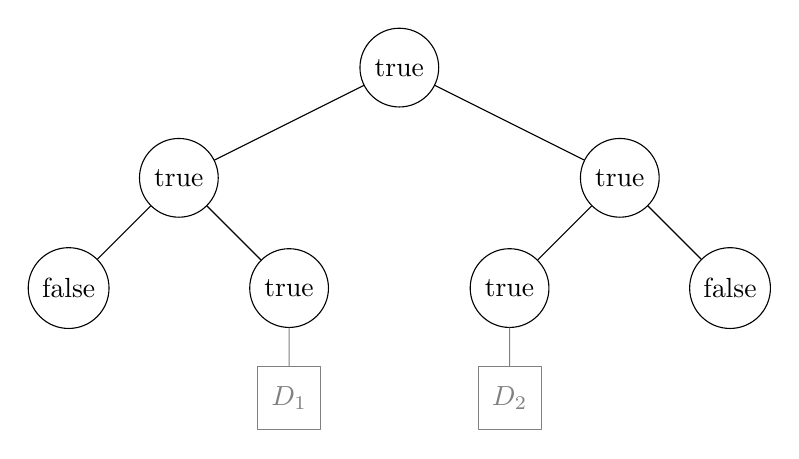
\begin{tikzpicture}[line cap=round, line join=round, scale=0.7]
						% First layer
						\node [circle, draw=black, fill=white, minimum size = 1cm] (node-1-1) at (0, 0) {true};
						% Second layer
						\foreach \a [count=\x] in {1, 2}
							\node [circle, draw=black, fill=white, minimum size=1cm] (node-2-\x) at (-12 + 8 * \x, -2) {true};
						% Third layer
						\node [circle, draw=black, fill=white, minimum size=1cm] (node-3-1) at (-6, -4) {false};
						\foreach \a in {2, 3}
							\node [circle, draw=black, fill=white, minimum size=1cm] (node-3-\a) at (-10 + 4 * \a, -4) {true};
						\node [circle, draw=black, fill=white, minimum size=1cm] (node-3-4) at (6, -4) {false};
						% First data layer
						\foreach \a [count=\x] in {1, 2}
							\node [draw=gray, text=gray, fill=white, minimum size=0.8cm] (data-1-\x) at (-6 + 4 * \x, -6) {$D_\a$};
						% First layer arrows
						\foreach \a in {1, 2}
							\draw (node-1-1) -- (node-2-\a);
						% Second layer arrows
						\foreach \a in {1, 2}
							\draw (node-2-1) -- (node-3-\a);
						\foreach \a in {3, 4}
							\draw (node-2-2) -- (node-3-\a);
						\draw [draw=gray] (node-3-2) -- (data-1-1);
						\draw [draw=gray] (node-3-3) -- (data-1-2);
					\end{tikzpicture}
					\caption{Representation.}
					\label{}
				\end{subfigure}
				\caption[Integrity Check: Array of Booleans]{The array of booleans and the corresponding representation for a multiple item proof with four data blocks, in which $D_1$ and $D_2$ should be verified.}
				\label{fig:mip-2}
			\end{figure}

			\begin{figure}
				\centering
				\begin{subfigure}[b]{0.4\linewidth}
					\centering
					$$
						[\textrm{\textcolor{gray}{null}}, \textrm{\textcolor{gray}{null}}, \textrm{\textcolor{gray}{null}}, H_3, \textrm{\textcolor{gray}{null}}, \textrm{\textcolor{gray}{null}}, H_6]
					$$
					\vspace*{3em}
					\caption{Data structure.}
					\label{}
				\end{subfigure}%
				\begin{subfigure}[b]{0.6\linewidth}
					\centering
					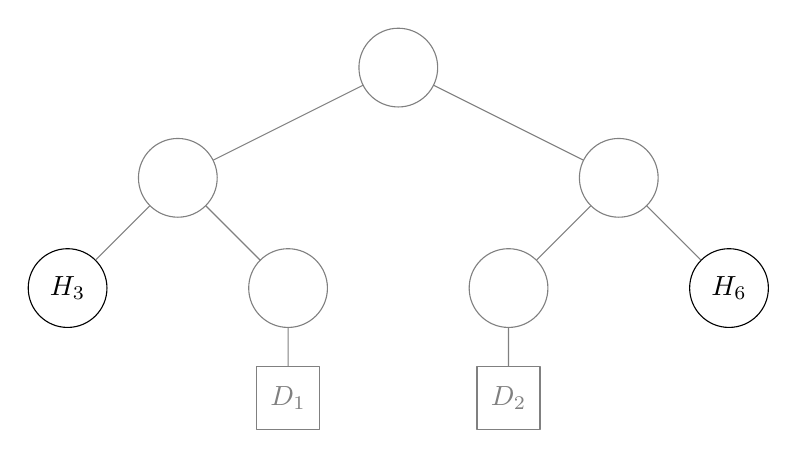
\begin{tikzpicture}[line cap=round, line join=round, scale=0.7]
						% First layer
						\node [circle, draw=gray, fill=white, minimum size = 1cm] (node-1-1) at (0, 0) {};
						% Second layer
						\foreach \a [count=\x] in {1, 2}
							\node [circle, draw=gray, fill=white, minimum size=1cm] (node-2-\x) at (-12 + 8 * \x, -2) {};
						% Third layer
						\node [circle, draw=black, fill=white, minimum size=1cm] (node-3-1) at (-6, -4) {$H_3$};
						\foreach \a in {2, 3}
							\node [circle, draw=gray, fill=white, minimum size=1cm] (node-3-\a) at (-10 + 4 * \a, -4) {};
						\node [circle, draw=black, fill=white, minimum size=1cm] (node-3-4) at (6, -4) {$H_6$};
						% First data layer
						\foreach \a [count=\x] in {1, 2}
							\node [draw=gray, text=gray, fill=white, minimum size=0.8cm] (data-1-\x) at (-6 + 4 * \x, -6) {$D_\a$};
						% First layer arrows
						\foreach \a in {1, 2}
							\draw [draw=gray] (node-1-1) -- (node-2-\a);
						% Second layer arrows
						\foreach \a in {1, 2}
							\draw [draw=gray] (node-2-1) -- (node-3-\a);
						\foreach \a in {3, 4}
							\draw [draw=gray] (node-2-2) -- (node-3-\a);
						\draw [draw=gray] (node-3-2) -- (data-1-1);
						\draw [draw=gray] (node-3-3) -- (data-1-2);
					\end{tikzpicture}
					\caption{Representation.}
					\label{}
				\end{subfigure}
				\caption[Integrity Check: Array of Hashes]{The array of hashes and the corresponding representation for a multiple item proof with four data blocks, in which $D_1$ and $D_2$ should be verified.}
				\label{fig:mip-3}
			\end{figure}

			\clearpage


		% Proof Verification
		\subsubsection{Proof Verification}
		\label{subsec:mip-verification}

			To verify a proof, the root hash for the respective Merkle tree has to be computed from the given proof data and compared to the stored root hash (see \autoref{subsec:merkle-tree}).
			\hyperref[alg:proof-verification]{Algorithm 1} shows the basic principle of the recursive root hash calculation in an off-chained smart contract.
			To get the hash for a node with index $i$, it is first determined using the array of booleans, whether the respective hash needs to be computed or is given in the array of hashes.
			If the hash is given, this is a base case of the recursion and the hash is simply returned (see \hyperref[algline:8]{line 8}).
			Otherwise, if $i$ is greater or equal to the index of the first leaf node, we know that the node with index $i$ has to be a leaf due to the level order in the underlying data structure (see \autoref{fig:mip-1}).
			This is also a base case of the recursion and the hash of the corresponding data block is returned (see \hyperref[algline:11]{line 11}).
			In all other cases, the hash needs to be recursively computed from the hashes of its children (see \hyperref[algline:15]{line 15}).
			This principle is used to compute the root hash (see \hyperref[algline:2]{line 2}), which is compared with the stored root hash.
			If the hashes are equal, the integrity of the off-chained data was successfully verified and the respective data blocks can be used in further computations.

			\begin{algorithm}
				\caption{Proof verification}
				\label{alg:proof-verification}

				\begin{algorithmic}[1]
					\Procedure{VerifyProof}{$booleans, hashes, dataBlocks, indexOfFirstLeaf$}
						\State $rootHash \gets \Call{ComputeHash}{0, booleans, hashes, dataBlocks, indexOfFirstLeaf}$ \label{algline:2}
						\If{$rootHash = storedRootHash$} \Return true \Comment{Proof is valid}
						\Else{} \Return false \Comment{Proof is invalid}
						\EndIf	
					\EndProcedure

					\State
					\Procedure{ComputeHash}{$i, booleans, hashes, dataBlocks, indexOfFirstLeaf$}
						\If{$booleans[i] = \textrm{false}$} \Comment{Hash does not need to be computed}
							\State \Return $hashes[i]$ \label{algline:8}
						\ElsIf{$i \geq indexOfFirstLeaf$} \Comment{Hash needs to be computed from a data block}
							\State $dataBlockIndex \gets i - indexOfFirstLeaf$ \Comment{Index of the data block}
							\State \Return $\textrm{hash}(dataBlock\ \textrm{with index}\ dataBlockIndex)$ \label{algline:11}
						\Else{} \Comment{Hash needs to be computed from children's hashes}
							\State $left \gets 2i + 1$ \Comment{Index of the left child}
							\State $right \gets 2i + 2$ \Comment{Index of the right child}
							\State \Return $\textrm{hash}(\Call{ComputeHash}{left, \dots} + \Call{ComputeHash}{right, \dots})$ \label{algline:15}
						\EndIf
					\EndProcedure
				\end{algorithmic}
			\end{algorithm}

			\clearpage
